%% ==== General ==============================================================

\newcommand{\authorName}{Jan Bulling}
\newcommand{\authorEmail}{jan.bulling@uni-ulm.de}
\newcommand{\matrikelnummer}{1109395}
\newcommand{\titleOfWork}{Title of the work}
\newcommand{\dateOfWork}{\today}
\newcommand{\subjectOfWork}{Bachelor Thesis}
\newcommand{\publisherOfWork}{Universität Ulm}
\newcommand{\institute}{Institute of Theoretical Physics}
\newcommand{\faculty}{Fakultät für\\Naturwissenschaften}
\newcommand{\supervisor}{Marit O. E. Steiner, Julen S. Pedernales, Martin B. Plenio}
% more: see sections/titlepage and section/titlepage_2


%% ===========================================================================
%% ===========================================================================
%% ===========================================================================
\documentclass[a4paper, 12pt,
bibliography=totoc,   %% references in contents
numbers=noenddot,     %% no point after last number in outline
% abstracton,         %% use abstract
% ngerman,            %% german (new-german)
% twocolumn,          %% two columns
% DIV9,               %% dividing paper into 9 parts
% BCOR7mm,            %% space on left for printing and binding
% twoside,            %% like a book but not using the book class
% chapterprefix,      %% the word "chapter" before each chapter
% headsepline,        %% line after heading (see footsepline)
captions=tableheading,  %% distance between table and text
]{scrreprt} %% srreprt for report (chapters) or scrartcl for article (sections,...), scrbook for book

\parindent 0pt	%% indent of new paragraphs
\parskip 6pt	%% distance between paragraphs

\pagestyle{headings} %% headings (empty, plain)


\interfootnotelinepenalty=10000 %% footnotes are not split between pages

\DeclareEmphSequence{\bfseries\itshape} %% \emph is bold and italic


%% --- fonts ---
\usepackage{lmodern}


%% --- language ---
% \usepackage[T1]{fontenc}
% \usepackage[utf8]{inputenc}
% \usepackage[ngerman]{babel}
\usepackage[english]{babel}


%% --- change font ---
% \usepackage[scaled]{helvet}
% \renewcommand{\familydefault}{\sfdefault} 
% \KOMAoptions{DIV=last}


%% --- graphics and images ---
\usepackage{graphicx}
\usepackage{color}

%% --- sub-figures ---
\usepackage[labelfont=bf]{caption}
\usepackage{subcaption}


%% --- math and physics ---
\usepackage{amsfonts, amssymb, amsmath, amsthm}
\usepackage{bbold} %% for \mathbb{1}
\usepackage{mathrsfs}   %% use scripting (\mathscr{A})
\numberwithin{equation}{chapter}    %% use chapter in equation numbering
\usepackage{physics}
\usepackage[version=4]{mhchem} %% chemical formulas (\ce{H_2O})
\usepackage{mathtools}  %% useful for \xrightarrow[Below]{Above}


%% footnotes keep counting and don't reset for each chapter
\counterwithout{footnote}{chapter}


%% --- Index ---- Usage: \index{word1}word1 - or -  \index{Abschlussarbeit!Bachelor!M. of Sc.}Abschlussarbeit
%% At correct position in the document: \printindex
% \usepackage{index}
% \makeindex


%% --- Acronym ---- Usage: \ac{USA}
% \usepackage[printonlyused,withpage]{acronym} 


%% --- Tikz and libraries ---
% \usepackage{tikz}

%% quantum circuits (https://mirrors.ibiblio.org/CTAN/graphics/pgf/contrib/quantikz/quantikz.pdf)
% \usetikzlibrary{quantikz2}


%% --- references --- Links and references in pdf document
\usepackage[
    % hidelinks,        %% hides colored links
    bookmarksopen=true, %% open bookmarks in e.g. Adobe reader
    bookmarksopenlevel=1,
    bookmarksnumbered=true,
    pdfusetitle,
    % pdfauthor={Jan Bulling},
    % pdfsubject={},
    % pdftitle={},
    % pdfkeywords={},
    % pdfproducer={Universität Ulm},
]{hyperref}

% \usepackage{varioref}   %% \vref for intelligent refs with page, \Vref for starting of sentence
\usepackage{cleveref}   %% \cref for intelligent refs


%% --- Tables ---
\usepackage{multirow}
\usepackage{array}
\usepackage{booktabs}
\newcolumntype{L}[1]{>{\raggedright\let\newline\\\arraybackslash\hspace{0pt}}m{#1}}
\newcolumntype{C}[1]{>{\centering\let\newline\\\arraybackslash\hspace{0pt}}m{#1}}
\newcolumntype{R}[1]{>{\raggedleft\let\newline\\\arraybackslash\hspace{0pt}}m{#1}}


%% --- Biblatex ---
%% (https://de.overleaf.com/learn/latex/Biblatex_bibliography_styles)
%% https://mirror.dogado.de/tex-archive/macros/latex/contrib/biblatex-contrib/biblatex-phys/biblatex-phys.pdf
\usepackage[]{csquotes}
\usepackage[
    backend=biber,
    style=phys,     %% phys, nature, numeric-comp, apa
    sorting=none,   %% none -> appearance, nty -> author, title, year, ...
    natbib=true,
    giveninits=true,
    abbreviate=false,
    block=space,
    %% biblatex-phys options
    url=false, isbn=false,
    doi=true, 
    eprint=true,
    biblabel=brackets
]{biblatex}
\addbibresource{./../Paper/bachelorarbeit.bib}


%% --- Custom commands ---
\newcommand{\q}[1]{``#1''}
\newcommand{\si}[1]{\, \mathrm{#1}}
\newcommand{\Si}[1]{\mathrm{#1}}

\renewcommand{\abs}[1]{\left\lvert#1\right\rvert}
\renewcommand{\norm}[1]{\left\lVert#1\right\rVert}
\newcommand{\mean}[1]{\left\langle#1\right\rangle}
% \newcommand{\mean}[1]{\overline{#1}}
\newcommand{\avg}[1]{\left\langle#1\right\rangle}
\renewcommand{\op}[1]{\hat{#1}}
\renewcommand{\deg}{\mathrm{^\circ}}

%% --- vector notations (leaf commented for default arrow) ----
\renewcommand{\Vec}[1]{\vectorbold{#1}}   %% bold font
% \renewcommand{\Vec}[1]{\bar{#1}}          %% overline
% \renewcommand{\Vec}[1]{\underline{#1}}    %% underline (Audenaert notation)
\renewcommand{\vec}[1]{\Vec{#1}}

%% --- Custom operators ---
\DeclareMathOperator{\diag}{diag}

%% --- Custom environments ---
%% usage: \begin{theorem}[Pythagorean theorem] ..... \end{theorem}
%% 
%% Definition: an explanation of the mathematical meaning of a word.
%% Theorem: A statement that has been proven to be true.
%% Proposition: A less important but nonetheless interesting true statement.
%% Lemma: A true statement used in proving other true statements (that is, a less important theorem that is helpful in the proof of other results).
%% Corollary: A true statement that is a simple deduction from a theorem or proposition.
\theoremstyle{plain}
\newtheorem{proposition}{Proposition}[chapter]
\newtheorem{theorem}{Theorem}[chapter]
\newtheorem{corollary}{Corollary}[chapter]
\newtheorem{lemma}[theorem]{Lemma}  %% shared counter with theorems

\theoremstyle{definition}
\newtheorem{definition}{Definition}[section]

\theoremstyle{remark}
\newtheorem*{remark}{Remark}    %% unnumbered

% \renewcommand{\qedsymbol}{$blacksquare$} %% redefine proof-end symbol



%% ===========================================================================
%% ===== Document ============================================================
%% ===========================================================================
\begin{document}

%% ---- title page ------------------------------------------------
%% choose title page (either sections/titlepage or sections/titlepage_2)
%\frontmatter
\thispagestyle{empty}

\begin{titlepage}
  \sffamily
  \raggedright

  \hfill
  
\includegraphics[height=1.8cm]{unilogo_sw.jpg}\\[2em]

  {\footnotesize
    \hspace*{115mm}
    \parbox[t]{35mm}{
      \bfseries \faculty\\

      \mdseries \institute
    }\\[2cm]
  
    \parbox{140mm}{\bfseries \LARGE \titleOfWork}\\[2.5em]
    {\bfseries \LARGE \subjectOfWork}\\[4em]

    {\footnotesize \bfseries Submitted by:}\\
    {\footnotesize \authorName\\ \authorEmail \\ \matrikelnummer} \\[2em]

    {\footnotesize \bfseries Supervised by:}\\
    {\footnotesize \supervisor}\\[2em]
  }
  
\end{titlepage}
  


% %% ===== Title page ==========================================

% multiple authors: Author 1\thanks{...} \and Author 2\thanks{...} \and ...
\author{\authorName \thanks{\authorEmail}}
\title{\titleOfWork}
\date{\dateOfWork}
\subject{\subjectOfWork}
\publishers{\publisherOfWork}

\titlehead{\hfill
\includegraphics[height=1.8cm]{unilogo_sw.jpg}}
%% back of title cover. Only if using a book class
% \uppertitleback{Back of title page}
% \lowertitleback{lower section after title page}

%% dedication on separate page
% \dedication{For my mom}

\maketitle[0]   %% in [] use the offset of the page number (can be negative)


%% ---- abstract ------------------------------------------------
\newpage
\begin{abstract}

In this work it was shown by calculating the relative dynamical phase build-up, that Casimir interactions between a conducting Faraday shield and macroscopic Schrödinger-cat states can destroy measurable entanglement due to stochastic variations in the initial setup and due to the thermal motion of the shield.
    
\end{abstract}


%% ---- table of contents, list of tables/figures ----------------
\newpage
\tableofcontents
% \listoffigures
% \listoftables

% ---- abbreviation --------------------------------------------
% \input{sections/acronym}


%% ---- content ------------------------------------------------
\newpage
\chapter{Introduction}\label{cha:introduction}




\section{Feynman's Gedankenexperiment}\label{sec:feynman-gedankenexperiment}


\chapter{A first look at the problem}\label{cha:first-look}

The quantum aspects of gravity can be tested with entanglement conveyed by gravitational interaction. A possible and naturally arising experiment to observe gravitationally induced entanglement is described in this chapter.
The rest of this thesis is about experimental issues with the descried procedure that are present in a real laboratory setting.

The experiment requires the ability to manipulate macroscopic massive bodies quantum mechanically by inducing a cat-state (a macroscopic spatial superposition state) or a squeezed state (!!!!!!!). 
This can be done in practice by e.g. utilizing a spin coupled to the center-of-mass motion of the object and a magnetic field gradient \cite{Bose_2017}. In the rest of this thesis I assume that all required states can be prepared.
Remarkable progress has been made in this field of quantum optomechanics in the last decade !!!SOURCES FROM E.G. ASPELMAYER!!!!.
Levitating the particles in a trap in a vacuum can increase environmental isolation by avoiding contact with surrounding noise. The additional forces due to the trapping can be well studied in advance.

The general problem is illustrated in \cref{fig:2:simple-problem}.
\begin{figure}[!htbp]
  \centering
  \def\svgwidth{\textwidth}
  \input{./../figures/simple-problem.pdf_tex}
  \caption{Schematic figure of the proposed experiment with two masses prepared in a spatial superposition state. The gravitational interaction $\op{H}$ induces different phases to each of the superpositions due to the different distances between all masses. This results in measurable entanglement after some time evolution.}
  \label{fig:2:simple-problem}
\end{figure}
Two bodies with masses $M_A$ and $M_B$ are suspended and prepared in a coherent quantum superposition Schrödinger-cat-like state with a separation of $\Delta x$.
Their center of masses are located a distance $2L$ away from each other.
For now, a setup is chosen as in \cref{fig:2:simple-problem}, where the superposition locations are aligned parallel to each other.
With the notation introduced in \cref{fig:2:simple-problem}, the initial state at $t=0$ is given by
\begin{equation}\label{eq:2:initial-state}
  \ket{\psi(t=0)} = \frac{1}{2}\left( \ket{\psi_A^1} + \ket{\psi_A^2} \right) \otimes \left( \ket{\psi_B^1} + \ket{\psi_B^2} \right) .
\end{equation}

The masses are assumed to interact only through their gravitational potential between each other. Any global factor of perturbation like the interaction with earth's gravitational field can be neglected. These kind of interactions manifests themselves only in a global phase factor for the evolved state.
For now, all other local interactions like Casimir-Polder \cite{Casimir_1948} or Coulomb forces are reduced to a minimum and are not considered at this stage.

The particles are assumed to be held in place by e.g. an optical trap and movement due to the gravitational acceleration is ignored on the time scales of the experiment. The Hamiltonian therefore only needs to include the gravitational interaction \footnote{In the low energy limit assumed here, relativistic effects do not play a role and the gravitational interaction between masses can be described by the classical Newtonian potential with the distance $D$ between masses replaced by an operator $\op{D}$.}, i.e.
\begin{equation}\label{eq:2:hamiltonian}
  \op{H} = \op{V} = -\frac{G M_A M_B}{\abs{\op{D}}},
\end{equation}
where $\op{D}$ is the distance operator between the masses depended on the individual positions $\op{x_A}$ and $\op{x_B}$.

During time evolution, the different superposition states build up different phases due to their different positions. I am interested whether this phase build-up results in measurable entanglement. This can, of cause, only happen if gravity is able to mediate entanglement.

\section{Time evolution under a gravitational potential}
The time evolution for a constant Hamiltonian $\op{H} = \op{V}(\op{x_i}) = \mathrm{const.}$ is governed by the Schrödinger equation
\begin{equation}
  i\hbar \pdv{t}\ket{\psi(t)} = \op{H} \ket{\psi(t)}
\end{equation}
with the general solution
\begin{equation}
  \ket{\psi(t)} = e^{-i \op{V} t / \hbar} \ket{\psi(t=0)} .
\end{equation}
By expressing $\op{V}$ and $\psi$ in the eigenbasis of the Hamiltonian like $\op{V}\ket{n} = V_n \ket{n}$ and $\ket{\psi(t=0)} = \sum c_n \ket{\psi_n}$, the time evolution is given in the very simple form
\begin{equation}
  \ket{\psi(t)} = \sum_n e^{-i V_n t /\hbar} c_n \ket{\psi_n} .
\end{equation}
Expressed in the $\left\{ \ket{\psi_A^1}, \ket{\psi_A^2} \right\}\otimes \left\{ \ket{\psi_B^1}, \ket{\psi_B^2} \right\}$ basis, the time evolution of the system in \eqref{eq:2:initial-state} described by the Hamiltonian from eq. \eqref{eq:2:hamiltonian} is thus given by
\begin{equation}\label{eq:2:evolved-state}
  \ket{\psi(t)} = \frac{1}{2}\bigl(
    e^{i\phi_{11}} \ket{\psi_A^1}\ket{\psi_B^1} 
    + e^{i\phi_{12}} \ket{\psi_A^1}\ket{\psi_B^2}
    + e^{i\phi_{21}} \ket{\psi_A^2}\ket{\psi_B^1} 
    + e^{i\phi_{22}} \ket{\psi_A^2}\ket{\psi_B^2} \bigr) ,
\end{equation}
where the $\otimes$ symbol between the states was omitted.
Here, the phases $\phi_{ij}$, $i,j \in \left\{1,2\right\}$ are
\begin{align}
  \phi_{11}=\phi_{22} = \frac{G M_A M_B}{2\hbar L}t 
  \qquad \text{and} \qquad 
  \phi_{12}=\phi_{21} = \frac{G M_A M_B}{\hbar \sqrt{4L^2 + (\Delta x)^2}}t.
\end{align}
Expanding the phases $\phi_{12} = \phi_{21} \approx G M_A M_B/\hbar \, \left[ 1/(2L) - (\Delta x)^2/(16L^3) \right] \equiv \phi_{11} - \Delta \phi$ a global phase $\phi_{12}$ can be factorized in eq. \eqref{eq:2:evolved-state} as
\begin{equation}
  \ket{\psi(t)} = \frac{1}{\sqrt{2}}e^{i\phi_{11}}\left[ 
    \ket{\psi_A^1} \otimes \frac{\ket{\psi_B^1} + e^{-i\Delta\phi} \ket{\psi_B^2}}{\sqrt{2}}
    + \ket{\psi_A^2} \otimes \frac{e^{-i\Delta\phi} \ket{\psi_B^1} + \ket{\psi_B^2}}{\sqrt{2}} \right] .
\end{equation}
The density matrix of this state expressed in the natural basis for the system is given by
\begin{equation}
  \rho(t) = \frac{1}{4}
  \begin{pmatrix}
    1 & e^{i\Delta\phi}  & e^{i\Delta\phi} & 1 \\
    e^{-i\Delta\phi} & 1 & 1  & e^{-i\Delta\phi} \\
    e^{-i\Delta\phi} & 1  & 1 & e^{-i\Delta\phi} \\
    1 & e^{i\Delta\phi} & e^{i\Delta\phi} & 1
  \end{pmatrix}.
\end{equation}
This state is entangled, if it cannot be represented in a product state $\ket{\psi} \neq \ket{\psi_A}\otimes\ket{\psi_B}$. Thus it is easy to see, that this condition is true if the two states multiplied by $\ket{\psi_A^i}$ not represent the same state i.e. they should not differ only by a phase factor.
The evolved state is therefore entangled, if $\Delta \phi \neq k\pi$ with integer $k \in \mathbb{Z}$.

%% FIDELITY
\section{Fidelity of quantum states}
In general, to compare the distance between two quantum states $\rho$ and $\sigma$ (\q{how similar they are}) the \emph{fidelity} $F(\rho, \sigma)$ is used. It is defined as \cite[p. 409-412]{Nielsen_2010} 
\begin{equation}
  F(\rho, \sigma) = \tr \sqrt{\sqrt{\rho} \sigma \sqrt{\rho}}
\end{equation} 
and can be used as a distance measurement between quantum states. It is monotonic, concave and bounded between 0 and 1. If both states are equal $\rho = \sigma$, it is clear that $F(\rho, \sigma) = 1$, by using $\sqrt{\rho}\rho\sqrt{\rho} = \rho^2$. If both states commute, i.e. they are diagonalizable in the same orthogonal basis $\{ \ket{i} \}$, 
\begin{equation*}
  \rho = \sum_i r_i \ketbra{i}; \quad \sigma = \sum_i s_i \ketbra{i},
\end{equation*}
the fidelity is given by \cite[p. 409]{Nielsen_2010}
\begin{equation*}
  F(\rho, \sigma) = \tr \sqrt{\sum_i r_i s_i \ketbra{i}} = \sum_i \sqrt{r_i s_i}.
\end{equation*}
This can be seen immediately by the use of the spectral theorem $\tr \sqrt{\rho} = \tr{U \sqrt{\mathrm{diag}(r_i)} U^\dagger} = \tr \diag(\sqrt{r_i})$.
Another special case is given for the fidelity of a pure state $\rho=\ketbra{\psi}$ and an arbitrary state $\sigma$ \cite[p. 409]{Nielsen_2010}:
\begin{equation*}
  F(\ket{\psi}, \sigma) = \tr \sqrt{\bra{\psi}\sigma\ket{\psi} \ketbra{\psi}} = \sqrt{\bra{\psi}\sigma\ket{\psi}}.
\end{equation*}
If the state $\sigma = \ketbra{\phi}$ is also pure, the fidelity reduces to
\begin{equation*}
  F(\ket{\psi}, \ket{\phi}) = \abs{\braket{\psi}{\phi}} \le 1,
\end{equation*}
with equality being attained if the states are the same and only differ by a phase. 

To quantify exactly how much the state $\psi(t)$ is entangled, a more sophisticated measurement for entanglement is necessary. In the next section, such a measurement - the \emph{logarithmic negativity} - is discussed and calculated for the present system.

\section{Entanglement measures}
To check whether an arbitrary state represented by a density matrix $\rho$ is entangled or not is no easy task. In fact, this problem is thought to be NP-hard \cite{Gurvits_2003}.






\begin{lemma}\label{lemma:trace-norm-hermitian}
  The trace norm $\norm{A}_1 \equiv \tr \sqrt{A^\dagger A}$ of a hermitian matrix $A$ is equal to the sum of the absolute eigenvalues of $A$.
\end{lemma}
\begin{proof}
  This can be immediately seen by the spectral theorem:
  \begin{equation*}
    \tr \sqrt{A^\dagger A} = \tr \sqrt{A^2} = \tr{U\sqrt{\diag(\lambda_1, \dots)^2}U^\dagger} = \sum_i \sqrt{\lambda_i^2} = \sum_i \abs{\lambda_i}.
  \end{equation*}
\end{proof}

\begin{proposition}\label{proposition:negativity}
  The \emph{negativity} $\mathscr{N}(\rho)$ of a state $\rho$ (defined below) is given as the absolute sum of all negative eigenvalues of $\rho$: 
\begin{equation}
    \mathscr{N}(\rho) \equiv \frac{\norm{\rho^{\Gamma_A}}_1 - 1}{2} = \abs{\sum_{\lambda_i < 0} \lambda_i}.
\end{equation}
\end{proposition}
\begin{proof}
  The proof is in parts given by Vidal \cite{Vidal_2001}. It is known that the density matrix is hermitian: $\rho = \rho^\dagger$. Using \cref{lemma:trace-norm-hermitian}, the trace norm of the density matrix is is given as $\norm{\rho}_1=\sum \lambda_i = \tr \rho = 1$. The partial transpose $\rho^{\Gamma_A}$ obviously also satisfies $\tr \rho^{\Gamma_A} = 1$ but might have negative eigenvalues. Since $\rho^{\Gamma_A}$ is still hermitian, the trace norm is given by
  \begin{equation*}
    \norm{\rho^{\Gamma_A}}_1 = \sum_i\abs{\lambda_i} = \sum_{\lambda_i \ge 0} \lambda_i + \sum_{\lambda_i < 0} \abs{\lambda_i} = \sum_i \lambda_i + 2\sum_{\lambda_i < 0} \abs{\lambda_i} = 1 + 2\sum_{\lambda_i < 0} \abs{\lambda_i} ,
  \end{equation*}
  where in the last step $\sum \lambda_i = \tr \rho^{\Gamma_A} = 1$ was used. The negativity can be defined as $\mathscr{N}(\rho) = \abs{\sum_{\lambda_i < 0} \lambda_i}$ and the statement is shown.
\end{proof}
\begin{remark}
  The method presented in \cref{proposition:negativity} is numerically more simple and requires zero matrix multiplications than to compute the sum of the square roots of the eigenvalues of $\rho^{\Gamma_A \dagger} \rho^{\Gamma_A}$ like shown in \cref{lemma:trace-norm-hermitian}. Furthermore in practice, $\rho^{\Gamma_A}$ has at most only one negative eigenvalue and numeric stability is increased by only taking a single value instead of summing over all eigenvalues.
\end{remark}
\begin{remark}
  The \emph{logarithmic negativity} \cite{Plenio_2005} relates to the negativity as follows
  \begin{equation}
    E_N(\rho) = \log_2 \norm{\rho^{\Gamma_A}}_1 = \log_2 \left( 2\mathcal{N}(\rho) + 1 \right)
  \end{equation}
  and can therefore be easily calculated by using the above \cref{proposition:negativity}. In comparison to the negativity, logarithmic negativity has additive properties \cite{Plenio_2005a}:
  \begin{equation*}
    E_N\left(\rho \otimes \sigma \right) = E_N(\rho) + E_N(\sigma) 
  \end{equation*}
\end{remark}




\section{Issues with the experimental procedure}


-------------------------


\section{Entanglement measures}
Why are they needed, what can one do?

Logarithmic negativity, properties, calculation





\begin{figure}[!htbp]
  \centering
  \def\svgwidth{0.9\textwidth}
  \input{./../figures/problem-geometry.pdf_tex}
  \caption{My problem}
\end{figure}


\begin{figure}[!htbp]
  \centering
  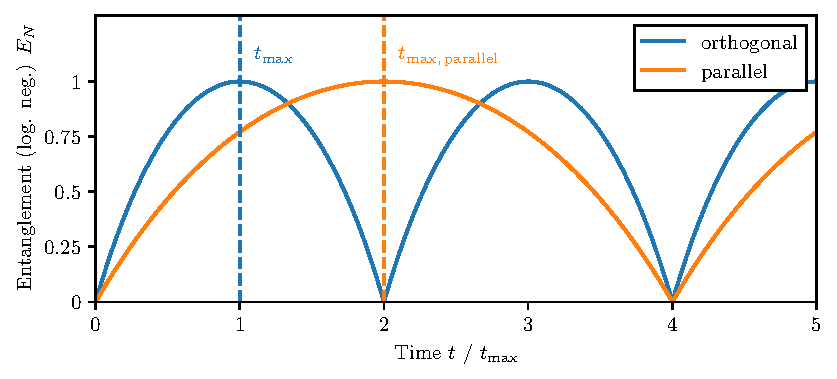
\includegraphics[width=\textwidth]{./../figures/EN-orientation-time.pdf}
  \caption{Entanglement dynamics quantified by the logarithmic negativity for two different orientations of the spatial superpositions relative to each other. The time of maximum entanglement $t_\mathrm{max}$ for the parallel configuration is given by $t_\mathrm{max} = 8\pi\hbar L^3 / (G M_A M_B d^2) \simeq 258\si{ms}$.}
\end{figure}
\chapter{Casimir effect}\label{cha:casimir-effect}

Casimir forces can be viewed in a very similar way to the \textit{van der Waals forces}. In fact, both phenomena describe just two different sides of the same coin. They define the so-called \emph{dispersion forces} between neutral atoms or bodies.
The quantum theory of van der Waals forces between two neutral atoms was developed by London in 1930 who found the attractive potential $\propto 1/r^6$ for small separations.
Casimir and Polder showed in 1948, that for separations larger than the resonance wavelength of the atoms, retardation effects need to be taken into account and the potential decays by a power law of $1/r^7$ \cite{Casimir_1948a}. 
Additionally, they calculated the interaction with a atom or molecule and a perfectly conducting wall, showing that macroscopic objects could experience these \emph{Casimir-Polder interactions} as well.
It becomes evident, that a full description of dispersion forces cannot be given by classical electrodynamics alone. Additional considerations regarding relativistic effects and quantum electrodynamics have to be made \cite{Bordag_2001,Klimchitskaya_2009,Lamoreaux_2004}.
Casimir, following a suggestion by Bohr \cite{Bordag_1999}, found a simple derivation using the zero-point energy of the vacuum to calculate the attraction between two conducting plates.
In quantum electrodynamics each point in the electromagnetic field can be described by an quantized harmonic oscillator with ground state energy $E_0 = \hbar\omega/2$.
The total \textit{zero-point energy} of the ground state of the field (the vacuum) is therefore given by summing over the energies $E_0$ for each possible mode $n$
\begin{equation}
  E_\mathrm{vacuum} = \frac{\hbar}{2} \sum_n \omega_n.
\end{equation} 
These sums are clearly divergent since there are infinitely many possible excitations.
Electrostatic boundary conditions require the field to be zero at the surface of the plate restricting the possible modes between the plates.
Precisely the finite difference between the infinite vacuum energy with and without the plates give rise to the \emph{Casimir forces} between two macroscopic objects.
A lot of textbooks are simply dropping the divergence motivated by the fact that energy is normally defined only up to a constant \cite{Bordag_2001}. 
Casimir was able to use regularization techniques to deal with the infinite quantities and arrived at his famous formula \cite{Casimir_1948}
\begin{equation}\label{eq:3:casimir-energy-pp-conducting}
  E_\mathrm{Casimir} = -\frac{\hbar c \pi^2}{720 L^3} A .
\end{equation}
for the attractive Casimir-potential between two plates with area $A$ and separation $L$.
The attractive force between the plates can now be simply expressed as
\begin{equation}\label{eq:3:casimir-force-pp-conducting}
  F_\mathrm{Casimir} = - \frac{\hbar c \pi^2}{240 L^4} A .
\end{equation}
It is remarkable, that such a simple relation arises out of the infinities of the vacuum.
Up until now, these Casimir forces are topic of modern scientific research. They are generally very difficult to calculate for other geometries than two infinitely large plates or for real materials with dielectric properties. 
Even for simple geometries, even the sign of the force is not always intuitively clear: As an example, the Casimir force can be repulsive for an ideal metal spherical shell \cite{Klimchitskaya_2009}.
For other simple and important bodies like the sphere-plane or sphere-sphere geometry, no universally valid formula for any separation between the bodies exists. This is discussed in more detail in \cref{sec:3:sphere-plate}.

Almost ten years after the discovery of Casimir and Polder, Lifshitz was the first to find an expression for the Casimir force between two dielectric plates with arbitrary relative permittivity $\varepsilon_{r,\,1,2}$ for separations larger than the resonant wavelength \footnote{The \q{resonance wavelength} for a macroscopic body in this case can be understood as e.g. the plasma frequency in the Drude model \cite{Ford_1998}. Different models for light-matter interaction result in slightly different resonant wavelength. The Lifshitz formula however holds true for the cases of separations in the micro-meter regime for all practical materials \cite{Kamp_2020}.} \cite{Lifshitz_1956}.
The expression he found facilitates the general complexity of the Casimir interactions and is only expressible as a complicated integral \cite{Lifshitz_1956}
\begin{multline}\label{eq:3:lifshitz-general-integral}
  F/A = -\frac{\hbar c}{32 \pi^2 L^4} \int_0^\infty \dd x \int_1^\infty \dd p \ \frac{x^3}{p^2}\biggl\{ \left[ \frac{(s_1+p)(s_2+p)}{(s_1-p)(s_2-p)} e^x - 1 \right]^{-1} + \\
  \left[ \frac{(s_1+ \varepsilon_{r,\,1} p)(s_2 + \varepsilon_{r,\,2} p)}{(s_1 - \varepsilon_{r,\,1} p)(s_2 - \varepsilon_{r,\,2} p)} e^x - 1 \right]^{-1} \biggr\}
\end{multline}
with
\begin{equation*}
  s_{1,2} = \sqrt{\varepsilon_{r,\,1,2} - 1 + p^2} .
\end{equation*}
In the limit of two perfectly conducting plates ($\varepsilon_{r,\,1} = \varepsilon_{r,\,2} \rightarrow \infty$), the integral can be solved analytically and one gets the same expression already obtained by Casimir
\begin{equation}
  F_\mathrm{cond.}/A = -\frac{\hbar c}{16 \pi^2 L^4} \int_0^\infty \dd x \int_1^\infty \dd p \ \frac{x^3}{p^2 (e^x - 1)} = -\frac{\hbar c \pi^2}{240 L^4} .
\end{equation}
Lifshitz determined the Casimir force between a conducting metal plate and a dielectric plate (denoted $\mathrm{DM}$) as well as the force between two dielectric plates with the same dielectric constant $\varepsilon_r$ ($\mathrm{DD}$) as
\begin{align} \label{eq:3:casimir-pp-F-DM-lifshitz}
  F_\mathrm{DM} &= -\frac{\hbar c \pi^2}{240 L^4} \frac{\varepsilon_r - 1}{\varepsilon_r + 1} \varphi(\varepsilon_r) \\
  F_\mathrm{DD} &= -\frac{\hbar c \pi^2}{240 L^4} \left( \frac{\varepsilon_r - 1}{\varepsilon_r + 1} \right)^2 \varphi(\varepsilon_r)\label{eq:3:casimir-pp-F-DD-lifshitz}
\end{align}
where $\varphi(\varepsilon_r)$ is a numerical function obtained by solving eq. \eqref{eq:3:lifshitz-general-integral}, which approaches $1$ for a perfect conductor. I calculated the function numerically and the result is shown in \cref{fig:3:lifshitz-function}.
\begin{figure}[!htbp]
  \centering
  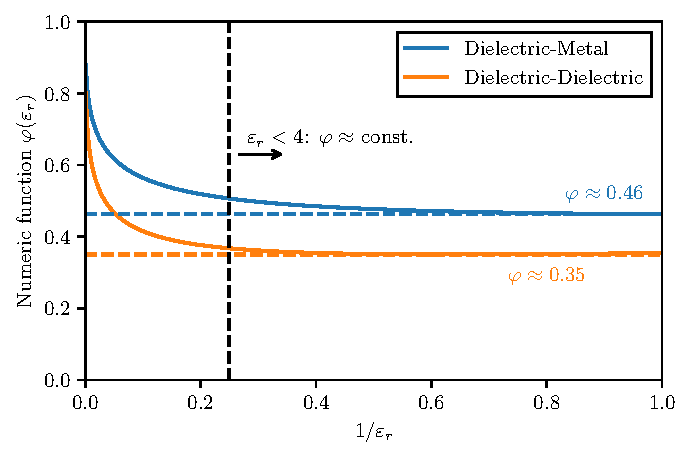
\includegraphics[width=0.8\textwidth]{./../figures/casimir-lifshitz-function.pdf}
  \caption{Numeric calculations of the function $\varphi(\varepsilon)$ used in the Lifshitz formula eq. \eqref{eq:3:casimir-pp-F-DM-lifshitz} and \eqref{eq:3:casimir-pp-F-DD-lifshitz}. The function was calculated for \textbf{(blue)} a dielectric and a metal plates and \textbf{(orange)} two dielectric plates. The function approaches unity for $\varepsilon\rightarrow\infty$ and a finite value for $\varepsilon\rightarrow 1$.}
  \label{fig:3:lifshitz-function}
\end{figure}
For a dielectric and metal plate, the function $\varphi$ approaches the finite value $\varphi(\varepsilon_r \rightarrow 1) \approx 0.46$ for small dielectric constants. However, this limit is practically already reached at $\varepsilon_r \approx 4$ and $\varphi$ stays approximately constant for smaller $\varepsilon_r$.



\section{Proximity force approximation}
\label{sec:3:pfa}

The Casimir-Polder force cannot be computed easily for different shapes. There even exists no analytic expression for the simple (and for this thesis relevant) plate-sphere geometry for all ratios $L/R$ and plate-sphere separations.
For a general shape, even the sign of the force, i.e. whether it is attractive or repulsive, is often unknown.
Fortunately, approximation methods exist and in particular the \emph{proximity-force-approximation (PFA)} can be calculated very easily \cite{Hartmann_2018,Emig_2007a,Bulgac_2006}.
The PFA is only valid for small separations ($L/R \approx 1$) between the considered smooth bodies.
The idea of this approximation is to divide the surfaces of the two bodies into infinitesimal small parallel plates with area $\dd A$ and summing over the forces $\dd F$ (or the Casimir-energy $\dd E$) between them (see \cref{fig:3:PFA}):
\begin{equation}\label{eq:3:pfa}
  E_\mathrm{PFA} = \iint_A \dd A \, \frac{E_\mathrm{plate-plate}}{A}
\end{equation}
where for the casimir energy per unit area $E_\mathrm{plate-plate}/A$ either eq. \eqref{eq:3:casimir-energy-pp-conducting} or any of the Lifshitz equations \eqref{eq:3:casimir-pp-F-DD-lifshitz}, \eqref{eq:3:casimir-pp-F-DM-lifshitz} can be chosen.
\begin{figure}[!htbp]
  \centering
  \def\svgwidth{0.55\textwidth}
  \input{./../figures/proximity-force-approximation.pdf_tex}
  \caption{In the proximity force approximation the sphere is divided into infinitesimal plane areas $\dd A$ which all exert a force $\dd F$ according to eq. \eqref{eq:3:casimir-force-pp-conducting}. All the contributions are added up together.}
  \label{fig:3:PFA}
\end{figure}
For the following calculations, it is important to distinguish between the distance between the plates center and the spheres center $L$ (like used before) and the edge-to-edge distance $\mathscr{L} = L - R$.

The problem with this approximation is, that it is ambiguous, what surface the area element $\dd A$ represents. For the plate-sphere geometry, the element can be either chosen tangential to the sphere or parallel to the plate (or in theory any other fictitious surface somewhere in between) \cite{Bulgac_2006}.
For the plate-sphere geometry, in the limit of the validity of the PFA $\mathscr{L} \ll R$ both methods yield the same result.
For the following calculations, I choose $\dd A$ parallel to the plate and the area can be parameterized with $r\in [0, R]$ and $\varphi \in [0, 2\pi]$ resulting in a distance $z$ between the infinitesimal area elements $z(r) = \mathscr{L} + R - \sqrt{R^2 - r^2}$ \footnote{Taking $\dd A$ tangential to the sphere, it can be parameterized with $\theta \in [0, \pi/2]$ and $\varphi \in [0, 2\pi]$ resulting in $z(\theta) = \mathscr{L} + R - R\cos\theta$. The PFA eq. \eqref{eq:3:pfa} yields with $\dd A = R^2\sin\theta\dd\theta\dd\varphi$ the result $\propto \frac{\pi R^2(R + 2\mathscr{L})}{\mathscr{L}^2(R+\mathscr{L})^2}$ which in the limit of $\mathscr{L} \ll R$ results in the same expression as eq. \eqref{eq:3:PFA-sphere-plate}.}. The PFA eq. \eqref{eq:3:pfa} then yields for a dielectric sphere against a perfectly conducting plate
\begin{align}
  E_\mathrm{plate-sphere} &= -\frac{\hbar c \pi^2}{720} \left(\frac{\varepsilon_r - 1}{\varepsilon_r + 1}\right) \varphi(\varepsilon_r) \int_0^R \dd r \int_0^{2\pi} r\dd \varphi \frac{1}{z(r)^3} \\
  &= -\frac{\hbar c \pi^3}{360} \left(\frac{\varepsilon_r - 1}{\varepsilon_r + 1}\right) \varphi(\varepsilon_r) \frac{R^2}{2\mathscr{L}^2(R + \mathscr{L})} \\
  &\approx -\frac{\hbar c \pi^3}{720} \left(\frac{\varepsilon_r - 1}{\varepsilon_r + 1}\right) \varphi(\varepsilon_r) \frac{R}{\mathscr{L}^2} \label{eq:3:PFA-sphere-plate}
\end{align}



\section{Imperfect plate and spheres}

Python numerical approach, gaussian modes (vibration modes of a spherical plane), perlin noise



\section{Casimir forces between a conducting plate and a dielectric sphere}
\label{sec:3:sphere-plate}

\subsection{Polarizability of a dielectric sphere}
The polarizability $\alpha$ is defined via
\begin{equation}
  \vec{E_\infty} \alpha = \vec{p},
\end{equation}
where $\vec{p}$ is the induced dipole moment and $\vec{E_\infty}$ is the external electric field that induces the dipole moment. For a linear and uniform dielectric, it is given as $\vec{p} = \mathcal{V} \varepsilon_0 (\varepsilon_r - 1) \vec{E_\mathrm{in}}$ \cite[p. 220-226]{Griffiths_2018}. Here, $\mathcal{V}$ is the volume of the object and $\vec{E_\mathrm{in}}$ is the electric field inside the dielectric.
The electrostatic boundary conditions for the problem are given by
\begin{equation}
  V_\mathrm{in} \big|_{r=R} = V_\mathrm{out} \big|_{r=R} 
  \quad \text{and} \quad 
  \varepsilon_r\varepsilon_0\pdv{V_\mathrm{in}}{r}\bigg|_{r=R} = \varepsilon_0\pdv{V_\mathrm{out}}{r} \bigg|_{r=R}
\end{equation}
and the electric potential outside of the sphere at $r\rightarrow\infty$ should be equal to the external dipole-inducing field $V_\mathrm{out} |_{r\rightarrow\infty} = -\vec{E_\infty} \cdot \vec{r} = -E_\infty r\cos\theta$.
The electric potential inside and outside the sphere can be calculated using the spherical decomposition of the general electric potential $V \propto 1/\abs{\vec{r} - \vec{r'}}$ into Legendre Polynomials $P_l$ \cite[p. 188-190]{Griffiths_2018}:
\begin{align}
  V_\mathrm{in}(r, \theta) &= -E_\infty r\cos\theta + \sum_{l=0}^{\infty} A_l r^l P_l(\cos\theta), \\
  V_\mathrm{out}(r, \theta) &= -E_\infty r \cos\theta + \sum_{l=0}^{\infty} \frac{B_l}{r^{l+1}} P_l(\cos\theta).
\end{align}
Applying both boundary conditions, it follows that \cite[p. 249-251]{Griffiths_2018}
\begin{equation}
  \begin{cases}
    A_l = B_l = 0 & \text{for } l \neq 1, \\
  A_1 = -\frac{3}{\varepsilon_r + 2}E_\infty, \quad B_1 = \frac{\varepsilon_r-1}{\varepsilon_r + 2}R^3E_\infty
  \end{cases}
\end{equation}
and the resulting  homogenous electric field $\vec{E_\mathrm{in}} = -\vec{\nabla} V_\mathrm{in}$ inside the sphere is given as
\begin{equation}
  \vec{E_\mathrm{in}} = \frac{3}{\varepsilon_r + 2} \vec{E_\infty} .
\end{equation}
The field is shown on the right in \cref{fig:dielectric-sphere-field}.The polarizability $\alpha$ of the sphere can be now be determined to
\begin{equation}
  \alpha_\mathrm{sphere} = 4\pi \varepsilon_0 R^3 \left(\frac{\varepsilon_r - 1}{\varepsilon_r + 2}\right).
\end{equation}

% \begin{figure}[!htbp]
%   \centering
%   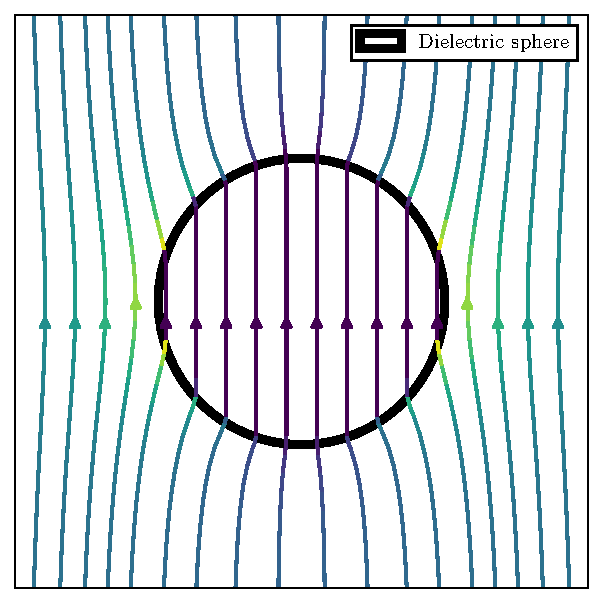
\includegraphics[width=0.8\textwidth]{./../figures/field-dielectric-sphere.pdf}
%   \label{fig:field-dielectric-sphere}
%   \caption{Electric field lines through an dielectric sphere}
% \end{figure}

\begin{figure}[!htbp]
  \centering
  \begin{subfigure}[b]{0.48\textwidth}
      \centering
      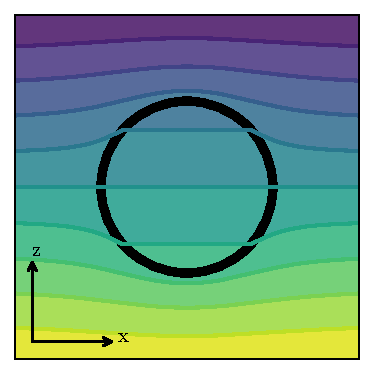
\includegraphics[width=\textwidth]{./../figures/potential-dielectric-sphere-small.pdf}
  \end{subfigure}
  \hfill
  \begin{subfigure}[b]{0.48\textwidth}
      \centering
      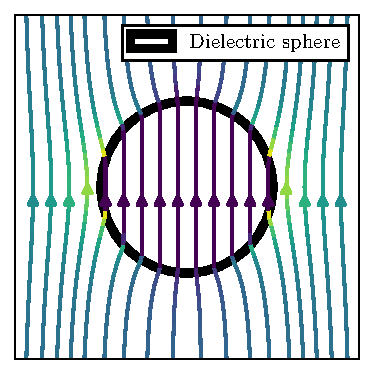
\includegraphics[width=\textwidth]{./../figures/field-dielectric-sphere-small.pdf}
  \end{subfigure}
  \caption{\textbf{left:} Electric potential $V$ of a dielectric sphere in a external electric field $\vec{E_\infty} \parallel \vec{e_z}$. \textbf{right:} The corresponding electric field lines inside and outside the dielectric sphere.}
  \label{fig:dielectric-sphere-field}
\end{figure}
\chapter{The shield}\label{cha:the-shield}

\begin{figure}[!htbp]
  \centering
  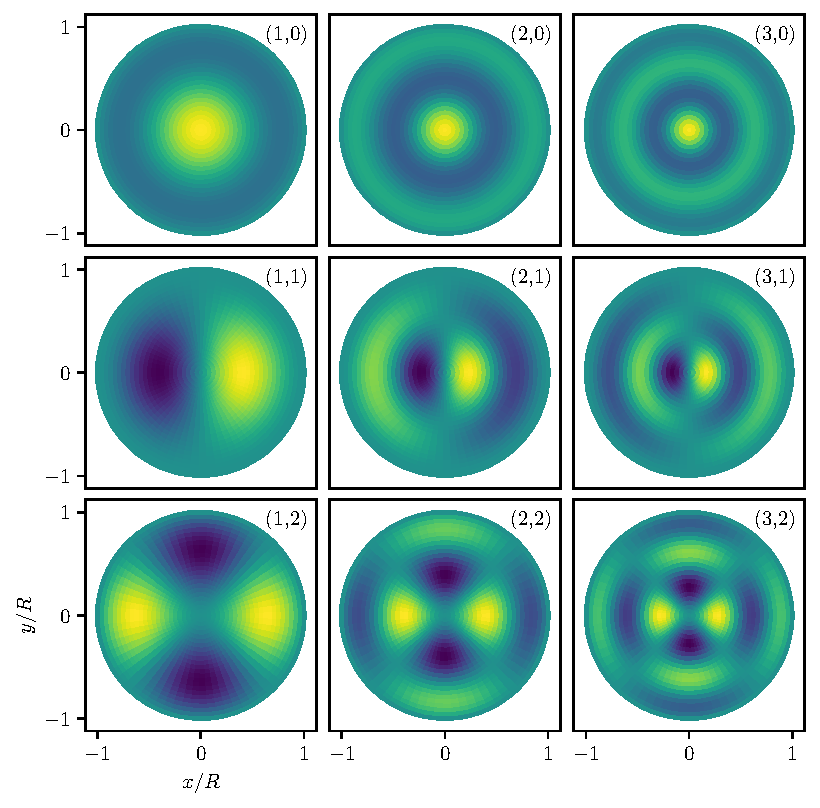
\includegraphics[width=\textwidth]{./../figures/vibrations/vibrational-modes.pdf}
  \label{fig:4:vibrational-modes}
  \caption{Vibrational modes of a spherical plate fixed at the edge with $R/d = 1000$.}
\end{figure}



Gravitational effect of the shield is neglectable
PROOF:





The modes $(k,l)$ have the shape
\begin{equation}
  u_{kl}(r, \theta, t) = A\left[J_k(\sqrt{\beta_l}r) - \frac{J_k(\sqrt{\beta_l}r_s)}{I_k(\sqrt{\beta_l}r_s)}I_k(\sqrt{\beta_l}r)\right]\cos(k\theta+\phi_1)\sin(\omega_{kl}t+\phi_2)
\end{equation}
with
\begin{equation}
  \beta_l = \frac{\tilde{x}_l^2}{r_s^2} \quad \quad \omega_{kl} = \frac{\tilde{x}_l^2}{r_s^2}\sqrt{\frac{D}{\rho d}} = \tilde{x}_l^2\frac{d}{r_s^2}\sqrt{\frac{E}{12\rho(1-\nu^2)}} ,
\end{equation}
where $\tilde{x}_l$ is the $l$-th solution of the equation
\begin{equation}
  J_k(\tilde{x}_l)I_{k+1}(\tilde{x}_l)+I_k(\tilde{x}_l)J_{k+1}(\tilde{x}_l) = 0 .
\end{equation}
The amplitude A of the vibrational mode $(k,l)$ is given by $A \sim \sqrt{\avg{x_{kl}^2}_T}$ where $\avg{x}$ is the variance of the oscillator mode
\begin{equation}
  \avg{x_{kl}^2}_T = \frac{\hbar}{2\tilde{m}\omega_{kl}} \coth(\frac{\hbar \omega_{kl}}{2 k_B T}) .
\end{equation}
Here, $\tilde{m}$ is the effective mass of the mode which depends on the shape of the mode. It can be calculated relative to the shield mass $m=\rho \pi r_s^2 d$ by
\begin{equation}
  \tilde{m} = m\frac{1}{\pi r_s^2}\int_0^{r_s} \dd r \int_0^{2\pi} r\dd\theta \, u_{kl}(r, \theta, t) .
\end{equation}

Shield vibrations can be understood like
\begin{equation}
  \alpha = \beta = \arctan{\max_{\substack{0 \leq r \leq r_s \\ \theta \in[0, 2\pi) \\ t \in [0,2\pi/\omega_{kl})}} \abs{\pdv{r}u_{kl}(r,\theta,t)}}
\end{equation}
and
\begin{align}
  \Delta L &= u_{kl}\left(\argmax_{\substack{0 \leq r \leq r_s \\ \theta, t}} \abs{\pdv{r}u_{kl}} \right) \lesssim \sqrt{\mean{x_{kl}^2}_T} \\
  &\approx \frac{1}{r_s} \left(r_s - \argmax_{0 \leq r \leq r_s}\abs{\pdv{r}u_{kl}}\right)\sqrt{\mean{x_{kl}^2}_T}
\end{align}


\begin{figure}[!htbp]
  \centering
  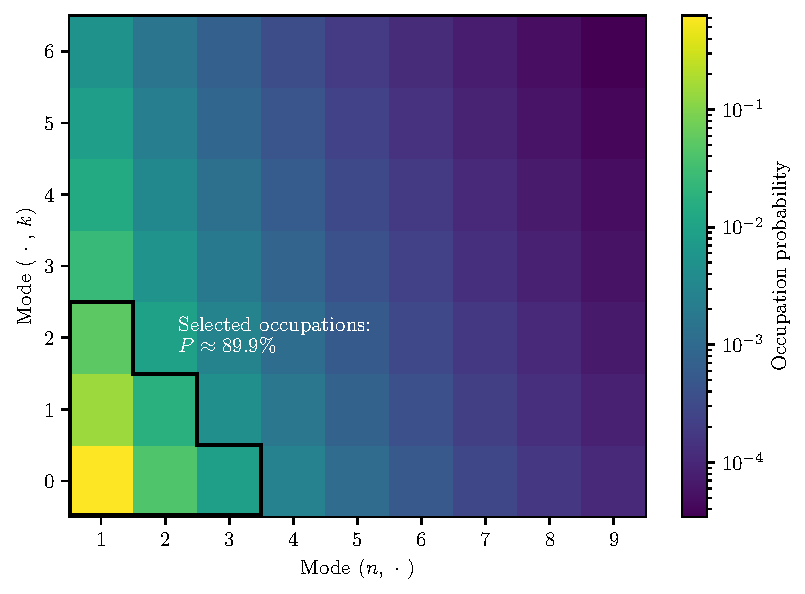
\includegraphics[width=\textwidth]{./../figures/vibrations/vibrations-mode-occupation.pdf}
  \label{fig:4:occupation-probability}
  \caption{Occupation probability of the modes at $T=4\si{K}$.}
\end{figure}
\chapter{The optimal setup}\label{cha:the-optimal-setup}


\begin{figure}[!htbp]
  \centering
  \def\svgwidth{0.9\textwidth}
  \input{./../figures/problem-geometry.pdf_tex}
  \caption{My problem}
\end{figure}


\section{Orientation}
$E_N$ depending on the orientation:

\begin{equation}
  E_N = \log_2\left\{
    1 + \abs{
      \sin(
      \frac{G M_A M_B t}{\hbar} \frac{\Delta x_A \Delta x_B}{8L^3}
      \left[ \sin\alpha\sin\beta - \frac{1}{2}\cos\alpha\cos\beta \right]
      )
      }
  \right\}
\end{equation}

Time till the maximum entanglement ($E_N = 1$):
\begin{equation}
  t_\mathrm{max} = \frac{8 \pi L^3 \hbar}{2 G M_A M_B \Delta x_A\Delta x_B} \abs{\sin\alpha\sin\beta - \frac{1}{2}\cos\alpha\cos\beta}^{-1}
\end{equation}

with a global minimum for $\alpha,\beta \in [0, \pi]$ for the orthogonal orientation with $\alpha = \beta = \pi/2$. Here, the time till the maximum entanglement is given by
\begin{equation}
  t_\mathrm{max} = \frac{4 \pi \hbar L^3}{G M_A M_B \Delta x_A \Delta x_B} \simeq 129\si{mn}
\end{equation}

\begin{figure}[!htbp]
  \centering
  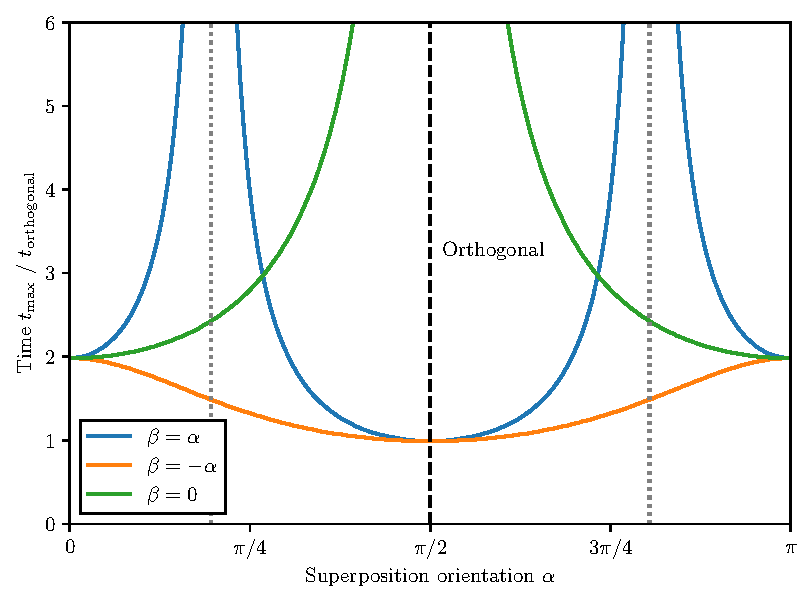
\includegraphics[width=\textwidth]{./../figures/ideal-entanglement/EN-orientation.pdf}
  \caption{...}
  \label{fig:5:optimal-orientation}
\end{figure}





%% ---- bibliography ------------------------------------------------
\newpage
\nocite{*}

\printbibliography

%% ---- appendix ------------------------------------------------
\appendix
\newpage

% \chapter{Proofs and other stuff}

\section{Negativity}

\begin{lemma}\label{lemma:trace-norm-hermitian}
  The trace norm $\norm{A}_1 \equiv \tr \sqrt{A^\dagger A}$ of a hermitian matrix $A$ is equal to the sum of the absolute eigenvalues of $A$.
\end{lemma}
\begin{proof}
  This can be immediately seen by the spectral theorem:
  \begin{equation*}
    \tr \sqrt{A^\dagger A} = \tr \sqrt{A^2} = \tr{U\sqrt{\diag(\lambda_1, \dots)^2}U^\dagger} = \sum_i \sqrt{\lambda_i^2} = \sum_i \abs{\lambda_i}.
  \end{equation*}
\end{proof}

\begin{proposition}\label{proposition:negativity}
  The \emph{negativity} $\mathscr{N}(\rho)$ of a state $\rho$ is given as the absolute sum of all negative eigenvalues of $\rho$: 
\begin{equation}
    \mathscr{N}(\rho) \equiv \frac{\norm{\rho^{\Gamma_A}}_1 - 1}{2} = \abs{\sum_{\lambda_i < 0} \lambda_i}.
\end{equation}
\end{proposition}
\begin{proof}
  The proof is in parts given by Vidal \cite{Vidal_2001}. It is known that the density matrix is hermitian: $\rho = \rho^\dagger$. Using \cref{lemma:trace-norm-hermitian}, the trace norm of the density matrix is is given as $\norm{\rho}_1=\sum \lambda_i = \tr \rho = 1$. The partial transpose $\rho^{\Gamma_A}$ obviously also satisfies $\tr \rho^{\Gamma_A} = 1$ but might have negative eigenvalues. Since $\rho^{\Gamma_A}$ is still hermitian, the trace norm is given by
  \begin{equation*}
    \norm{\rho^{\Gamma_A}}_1 = \sum_i\abs{\lambda_i} = \sum_{\lambda_i \ge 0} \lambda_i + \sum_{\lambda_i < 0} \abs{\lambda_i} = \sum_i \lambda_i + 2\sum_{\lambda_i < 0} \abs{\lambda_i} = 1 + 2\sum_{\lambda_i < 0} \abs{\lambda_i} ,
  \end{equation*}
  where in the last step $\sum \lambda_i = \tr \rho^{\Gamma_A} = 1$ was used. The negativity can be defined as $\mathscr{N}(\rho) = \abs{\sum_{\lambda_i < 0} \lambda_i}$ and the statement is shown.
\end{proof}
\begin{remark}
  The \emph{logarithmic negativity} \cite{Plenio_2005} relates to the negativity as follows
  \begin{equation}
    E_N(\rho) = \log_2 \norm{\rho^{\Gamma_A}}_1 = \log_2 \left( 2\mathcal{N}(\rho) + 1 \right)
  \end{equation}
  and can therefore be easily calculated by using the above \cref{proposition:negativity}. In comparison to the negativity, logarithmic negativity has additive properties \cite{Plenio_2005a}:
  \begin{equation*}
    E_N\left(\rho \otimes \sigma \right) = E_N(\rho) + E_N(\sigma) 
  \end{equation*}
\end{remark}

\newpage

%%%% ---------- Variant 2 ---------------
% \begin{proposition}\label{theorem:negativity}
% The \emph{negativity} $\mathscr{N}(\rho)$ of a state $\rho$ is given as the absolute sum of all negative eigenvalues of $\rho$: 
% \begin{equation}
%   \mathscr{N}(\rho) \equiv \frac{\norm{\rho^{\Gamma_A}}_1 - 1}{2} = \abs{\sum_{\lambda_i < 0} \lambda_i}
% \end{equation}
% \end{proposition}

% \begin{proof}
%   The proof is given in two steps, which in parts is given by Vidal \cite{Vidal_2001}:
% \begin{enumerate}
%   \item It is known, that the density matrix is hermitian: $\rho^\dagger = \rho$. For a general hermitian matrix $A$, the trace norm $\norm{A}_1 \equiv \tr \sqrt{A^\dagger A}$ is equal to the sum of the absolute eigenvalues of A.
%   This can be immediately seen by the spectral theorem:
%   \begin{equation*}
%     \tr \sqrt{A^\dagger A} = \tr \sqrt{A^2} = \tr{U\sqrt{\diag(\lambda_1, \dots)^2}U^\dagger} = \sum_i \sqrt{\lambda_i^2} .
%   \end{equation*}
%   \item The trace norm of the density matrix is given as $\norm{\rho}_1=\sum \lambda_i = \tr \rho = 1$. The partial transpose $\rho^{\Gamma_A}$ obviously also satisfies $\tr \rho^{\Gamma_A} = 1$ but might have negative eigenvalues. Since $\rho^{\Gamma_A}$ is still hermitian, the trace norm is given by
%   \begin{equation*}
%     \norm{\rho^{\Gamma_A}}_1 = \sum_i\abs{\lambda_i} = \sum_{\lambda_i \ge 0} \lambda_i + \sum_{\lambda_i < 0} \abs{\lambda_i} = \sum_i \lambda_i + 2\sum_{\lambda_i < 0} \abs{\lambda_i} = 1 + 2\sum_{\lambda_i < 0} \abs{\lambda_i} ,
%   \end{equation*}
%   where in the last step $\sum \lambda_i = \tr \rho^{\Gamma_A} = 1$ was used. The negativity can be defined as $\mathscr{N}(\rho) = \abs{\sum_{\lambda_i < 0} \lambda_i}$ and the statement is shown.
% \end{enumerate}
% \end{proof}
% \begin{remark}
%   The \emph{logarithmic negativity} \cite{Plenio_2005} relates to the negativity as follows
%   \begin{equation}
%     E_N(\rho) = \log_2 \norm{\rho^{\Gamma_A}}_1 = \log_2 \left( 2\mathcal{N}(\rho) + 1 \right)
%   \end{equation}
%   and can therefore be easily calculated by using the above \cref{theorem:negativity}. In comparison to the negativity, logarithmic negativity has additive properties \cite{Plenio_2005a}:
%   \begin{equation*}
%     E_N\left(\rho \otimes \sigma \right) = E_N(\rho) + E_N(\sigma) 
%   \end{equation*}
% \end{remark}




\section{Fidelity}
The \emph{fidelity} of two quantum states $\rho$ and $\sigma$ is defined as \cite[p. 409-412]{Nielsen_2010} 
\begin{equation}
  F(\rho, \sigma) = \tr \sqrt{\sqrt{\rho} \sigma \sqrt{\rho}}
\end{equation}
and can be used as a distance measurement between quantum states. It is monotonic, concave and bounded between 0 and 1. If both states are equal $\rho = \sigma$, it is clear that $F(\rho, \sigma) = 1$, by using $\sqrt{\rho}\rho\sqrt{\rho} = \rho^2$. If both states commute, i.e. they are diagonalizable in the same orthogonal basis $\{ \ket{i} \}$, 
\begin{equation*}
  \rho = \sum_i r_i \ketbra{i}; \quad \sigma = \sum_i s_i \ketbra{i},
\end{equation*}
the fidelity is given as \cite{Nielsen_2010}
\begin{equation*}
  F(\rho, \sigma) = \tr \sqrt{\sum_i r_i s_i \ketbra{i}} = \sum_i \sqrt{r_i s_i}.
\end{equation*}
This can be seen immediately by the use of the spectral theorem $\tr \sqrt{\rho} = \tr{U \sqrt{\mathrm{diag}(r_i)} U^\dagger} = \tr \diag(\sqrt{r_i})$.
Another special case is given for the fidelity of a pure state $\rho=\ketbra{\psi}$ and an arbitrary state $\sigma$ \cite{Nielsen_2010}:
\begin{equation*}
  F(\ket{\psi}, \sigma) = \tr \sqrt{\bra{\psi}\sigma\ket{\psi} \ketbra{\psi}} = \sqrt{\bra{\psi}\sigma\ket{\psi}}.
\end{equation*}
If the state $\sigma = \ketbra{\phi}$ is also pure, the fidelity reduces to
\begin{equation}
  F(\ket{\psi}, \ket{\phi}) = \abs{\braket{\psi}{\phi}} \le 1,
\end{equation}
with equality being attained if the states are the same and only differ by a phase. 
\chapter{TITLE TO BE DONE}
\section{Evolution under a gravitational Hamiltonian}
In this section the time evolution of a system under Hamiltonian eq. \eqref{eq:2:general-hamiltonian} is calculated a) using the gravitational interaction $\op{H}_G$ as a perturbation b) using an exact time evolution of coherent states.

\subsection{Using time dependent perturbation theory}
\label{apx:general-state-perturbation-theory}
A general biparty Fock state $\ket{\psi_0} = \ket{kl}$ with $k, l \in \mathbb{N}_0$ can be evolved in time under a Hamiltonian eq. \eqref{eq:2:general-hamiltonian} treating the gravitational interaction $H_G = -\hbar g (\op{a}_1\op{a}_2^\dagger + \op{a}_1^\dagger\op{a}_2)$ as a perturbation. 
The resulting state $\ket{\psi(t)}$ after some time $t$ is in the most general form given as
\begin{equation}
  \ket{\psi(t)} = \sum_{i, j \geq 0} c_{i,j}(t) \ket{i,j}
\end{equation}
where the coefficients $c_{i,j}(t)$ are given by first order perturbation theory as
\begin{equation}
  c_{i,j}(t) = c_{i,j}(t = 0) - \frac{i}{\hbar} \int_0^t \dd t' \bra{ij}\op{H}_G\ket{kl} e^{-i(E_{kl}-E_{ij})t'/\hbar} .
\end{equation}
The exponent is given by the energy of the appropriate Fock states $E_{kl}-E_{ij} = \hbar \omega (k+l - (i+j))$ and the matrix element in the integrand can be calculated to
\begin{equation}
  \bra{ij}\op{H}_G\ket{kl} =
  \begin{cases}
    -\hbar g & \text{if } i = k \pm 1 \text{ and } j = l \mp 1 \\
    0 & \text{otherwise}
  \end{cases}.
\end{equation}
The coefficients for $t=0$ are trivially given from the initial state as
\begin{equation}
  c_{i,j}(t=0) = \begin{cases}
    1 & \text{for } i,j = k,l \\
    0 & \text{otherwise}
  \end{cases}.
\end{equation}
For the non-zero states the energies in the exponent equate to zero and the evolved state is given by (up to a normalization)
\begin{equation}\label{eq:apx:perturbation-result}
  \ket{\psi(t)} = \ket{kl} - i g t \ket{k-1,l+1} - i g t \ket{k+1,l-1} + \mathcal{O}(g^2).
\end{equation}
The result eq. \eqref{eq:2:general-evolved-state} is represented by eq. \eqref{eq:apx:perturbation-result} for the case of $k=1$ and $l=0$.


\subsection{Using an exact time evolution}
\label{apx:general-coherent-state-evolution}
The Hamiltonian eq. \eqref{eq:2:general-hamiltonian} can be rewritten using symmetric and antisymmetric normal modes
\begin{equation}
  \op{a}_\pm = \frac{1}{\sqrt{2}} \left( \op{a}_1 \pm \op{a}_2 \right)
\end{equation}
in the form of 
\begin{equation}
  \op{H} = \hbar \omega_+ \op{a}^\dagger_+\op{a}_+ + \hbar \omega_- \op{a}^\dagger_-\op{a}_- ,  \quad  \omega_\pm = \omega \pm (-g)
\end{equation}
The initial state consisting of two coherent oscillator states is in the new modes given by
\begin{equation}\label{eq:apx:coherent-initial-state}
  \ket{\psi(t)} = \ket{\alpha}_1\ket{\beta}_2 = \ket{\frac{1}{\sqrt{2}} (\alpha + \beta)}_+\ket{\frac{1}{\sqrt{2}} (\alpha - \beta)}_-
\end{equation}
A general coherent state $\ket{\gamma}$ evolves in time under an Hamiltonian $\op{H} = \hbar \omega \op{a}^\dagger \op{a}$ like $\ket{\gamma(t)} = \ket{e^{-i\omega t} \gamma}$ which can be used to evolve the state in eq. \eqref{eq:apx:coherent-initial-state}:
\begin{align}
  \ket{\psi(t)} 
  &= \ket{ \frac{1}{\sqrt{2}} e^{-i\omega_+t} (\alpha + \beta) }_+\ket{ \frac{1}{\sqrt{2}} e^{-i\omega_-t} (\alpha - \beta) }_- \\
  &= \ket{ e^{-i\omega t} \left( \alpha \cos gt - \beta \sin gt \right) }_1 \ket{ e^{-i\omega t} \left( - \alpha \sin gt + \beta \cos gt \right) }_2, 
\end{align}
where in the last line the back-transformation from the $\pm$-modes \eqref{eq:apx:coherent-initial-state} was used.


\section{Exemplary calculation of $E_N$}
\label{apx:E_N-exemplary}
In this section, the logarithmic negativity $E_N$ eq. \eqref{eq:2:logarithmic-negativity} is exemplary calculated for the state eq. \eqref{eq:2:evolved-state}.
The density matrix of this system is given by
\begin{equation}
  \rho(t) = \ketbra{\psi(t)} = \frac{1}{4}
  \begin{pmatrix}
    1 & e^{i\Delta\phi}  & e^{i\Delta\phi} & 1 \\
    e^{-i\Delta\phi} & 1 & 1  & e^{-i\Delta\phi} \\
    e^{-i\Delta\phi} & 1  & 1 & e^{-i\Delta\phi} \\
    1 & e^{i\Delta\phi} & e^{i\Delta\phi} & 1
  \end{pmatrix}.
\end{equation}
Consequently, the partially transposed density $\rho^{\Gamma_B}$ is given by
\begin{equation}
  \rho^{\Gamma_B}(t) = \frac{1}{4}
  \begin{pmatrix}
    1 & e^{-i\Delta\phi}  & e^{i\Delta\phi} & 1 \\
    e^{i\Delta\phi} & 1 & 1  & e^{-i\Delta\phi} \\
    e^{-i\Delta\phi} & 1  & 1 & e^{i\Delta\phi} \\
    1 & e^{i\Delta\phi} & e^{-i\Delta\phi} & 1
  \end{pmatrix}.
\end{equation}
The eigenvalues where calculated using \texttt{Mathematica} and equate to
\begin{equation*}
  \left\{ \sin^2\left(\frac{\Delta\phi}{2}\right), \cos^2\left(\frac{\Delta\phi}{2}\right), \frac{\sin\Delta\phi}{2}, -\frac{\sin\Delta\phi}{2} \right\}
\end{equation*}
According to \cref{lemma:trace-norm-hermitian}, $\norm{\rho^{\Gamma_B}}_1$ is given by the sum of the absolute eigenvalues, which is equal to $1+\abs{\sin\Delta\phi}$. The negativity as the absolute sum of all negative eigenvalues (demonstrated in \cref{proposition:negativity}) equates to $\mathcal{N} = \abs{\sin\Delta\phi}/2$. Both methods result in a logarithmic negativity of $E_N = \log_2(1 + \abs{\sin\Delta\phi})$.


%% ---- index --------------------------------------------------
% \printindex

\end{document}
